\section{Particle Filters}
\label{particle_filters}

Gaussian filtering is a useful technique in order to perform nonlinear filtering. Popular techniques that 
use Gaussian filtering are the   the extended and unscented Kalman filtering. However, these methods do not perform well when

\begin{itemize}
\item The models are highly nonlinear
\item When the posterior distribution is significantly non-Gaussian e.g. a multimodal density
\end{itemize}


For these kinds of problems we need a different type of approximation to the posterior density. One such approach is the particle filter
method that we will discuss in this section, see \cite{Thurn2002} for a short introduction. 


The idea behind this filtering technique is  to aquire point-wise
estimates, called samples, of the posterior $p(\mathbf{x}_k | \mathbf{y}_{1:k})$. Then, as the number of samples increases,
the accuracy of the approximation increases. 

\section{Introduction to Particle Filtering }
\label{particle_filter_introduction}

Particle filters have solved several hard perceptual problems in robotics. Concretely, particle filters were able to solve
two important problmes; the global localization problem and the kidnapped robot problem, see \cite{Thurn2002} and references therein.
Another example where the particle filters approach is used successfully is the simultaneous localization and mapping (SLAM) problem \cite{Thurn2002}.
In particular, FastSLAM has been demonstrated to solve problems with more than 100000 dimensions in real-time \cite{Thurn2002}. 

\begin{framed}
\begin{remark}{\textbf{Kidnapped Robot Problem}}

In this problem a robot has to recover its pose under global uncertainty \cite{Thurn2002}.
\end{remark}
\end{framed}

\begin{framed}
\begin{remark}{\textbf{Global Localization  Problem}}
\end{remark}
\end{framed}
 
Particle filters are numerical techniques for approximating posterior probabilities in partially observable controllable Markov 
chains with discrete time \cite{Thurn2002}. Concretely, particle filters comprise a broad family of sequential Monte Carlo algorithms
for probability approximation in such environments.

\begin{framed}
\begin{remark}{\textbf{Partially Observable Markov Chains}}
\end{remark}
\end{framed}

\begin{framed}
\begin{remark}{\textbf{Sequential Monte Carlo}}

Particle filters are also known as sequential importance resampling or sequential Monte Carlo.
The basis of these methods is an algorithm called  sequential importance sampling, see section \ref{sequential_importance_sampling}. 
\end{remark}
\end{framed}

\subsection{Mathematical Formulation}
\label{pf_mathematical_formulation}

Let us assume that the state of a Markov chain at time $t$ is $\mathbf{x}_t$ and it depends on the
state at time $t-1$, $\mathbf{x}_{t-1}$ and the control input $\mathbf{u}_t$ according to the so called \textbf{motion model}, see \cite{Thurn2002}, 

\begin{equation}
p(\mathbf{x}_t | \mathbf{x}_{t-1}; \mathbf{u}_{t}) 
\label{pf_motion_model}
\end{equation}

It is assumed that the only information we have about the state of the environment at time $t$ is the measurement $\mathbf{z}_t$
whci is a probabilistic projection of the true state $\mathbf{x}_t$. It is generated according to the so called \textbf{measurement model}

\begin{equation}
p(\mathbf{z}_t | \mathbf{x}_{t}) 
\label{pf_measurement_model}
\end{equation}

Also let us assume that the  initial state $\mathbf{x}_0$ is described by the distribution $p(\mathbf{x}_0)$ i.e.
\begin{equation}
\mathbf{x}_0 \sim p(\mathbf{x}_0)
\end{equation}

The basic idea behind particle filtering is to use a non-parametric representation of the posterior

\begin{equation}
p(\mathbf{x}_k | \mathbf{y}_{1:k}) \approx \sum_{i=1}^N w_{k}^{(i)} \delta (\mathbf{x}_k -\mathbf{x}_{k}^{(i)})
\end{equation}

where $\mathbf{x}_{k}^{(i)}$ are particles and $w_{k}^{(i)}$ are associated weights.

We can then perform filtering by propagating $\mathbf{x}_{k}^{(i)}$ over time and
updating the weights.


\subsection{Monte Carlo sampling}
\label{monte_carlo_sampling}

Given independent samples $\mathbf{x}^{(1)}, \mathbf{x}^{(2)}, \ldots, \mathbf{x}^{(N)} \sim p(\mathbf{x})$ we can approximate

\begin{eqnarray}
E[\mathbf{g}(\mathbf{x})] \approx \frac{1}{N}\sum_{i=1}^N \mathbf{g}(\mathbf{x}^{(i)}) \\
p(\mathbf{x}) \approx \frac{1}{N}\sum_{i=1}^N \delta(\mathbf{x} - \mathbf{x}^{(i)})
\end{eqnarray}

Monte Carlo approximations have the following characteristics

\begin{itemize}
\item Non-parametric approximation to $p(\mathbf{x})$
\item Approximates all kinds of densities $p(\mathbf{x})$
\item Does not suffer from the curse of dimensionality
\end{itemize}

\begin{framed}
\theoremstyle{remark}
\begin{remark}{\textbf{Curse of Dimensionality}}

\end{remark}
\end{framed}

However, we should note that it is often difficult to generate samples from $p(\mathbf{x})$

\subsection{Importance sampling}
\label{importance_sampling}

Importance sampling can be used when it is difficult to sample from $p(\mathbf{x})$. Importance sampling generates samples
$\mathbf{x}^{(1)}, \mathbf{x}^{(2)}, \ldots, \mathbf{x}^{(N)}$ from a a proposal density $q(\mathbf{x})$. We can then set $p(\mathbf{x})$ as

\begin{equation}
p(\mathbf{x}) \approx \sum_{i=1}^N w^{(i)} \delta (\mathbf{x} -\mathbf{x}^{(i)})
\end{equation} 

where the weights are given by

\begin{equation}
w^{(i)} = \frac{\tilde{w}^{(i)}}{\sum_{n=1}^N \tilde{w}^{(i)}}, ~~ \tilde{w}^{(i)} = \frac{p(\mathbf{x}^{(i)})}{q(\mathbf{x}^{(i)})}
\end{equation}

Importance sampling is a flexible and powerful tool. It performs well as long as

\begin{itemize}
\item It is easy to sample from $q(\mathbf{x})$
\item The support of $q(\mathbf{x})$ contains the support of $p(\mathbf{x})$
\item $q(\mathbf{x})$ is similar to $p(\mathbf{x})$
\end{itemize}

\subsection{Sequential Importance Sampling (SIS)}
\label{sequential_importance_sampling}

Recall that our goal is to recursively and accurately approximate the filtering density $p(\mathbf{x}_k | \mathbf{y}_{1:k})$.
In order to do so we assumed that both the motion and measurement models, i.e. $p(\mathbf{x}_k | \mathbf{x}_{k-1})$ and $p(\mathbf{y}_k | \mathbf{x}_{k})$
respectively, can be evaluated point-wise. For example, for the model 

\begin{eqnarray}
\mathbf{x}_k = f(\mathbf{x}_{k-1}) + \mathbf{q}_{k-1}, ~~ \mathbf{q}_{k-1} \sim N(\mathbf{0}, \mathbf{Q}_{k-1}) \\
\mathbf{y}_k = h(\mathbf{x}_{k-1}) + \mathbf{r}_{k-1}, ~~ \mathbf{r}_{k-1} \sim N(\mathbf{0}, \mathbf{R}_{k-1}) 
\end{eqnarray}
then the density 

\begin{equation}
p(\mathbf{x}_k | \mathbf{x}_{k-1}) = N(\mathbf{x}_k; f(\mathbf{x}_{k-1}), \mathbf{Q}_{k-1})
\end{equation}

is generally easy to be evaluated for any values of $ \mathbf{x}_k$ and $\mathbf{x}_{k-1}$.

Particle filters are also known as sequential importance resampling or sequential Monte Carlo.
The basis of these methods is an algorithm called  sequential importance sampling. The standard SIS algorithm
is outlined below 


\begin{framed}
\theoremstyle{remark}
\begin{remark}{\textbf{Standard SIS Algorithm}}

\begin{enumerate}
\item For $i=1,\ldots, N$ at each time $k$ do:
	\begin{itemize}
		\item Draw $\mathbf{x}_{k}^{(i)} \sim q(\mathbf{x}_k | \mathbf{x}_{k-1}^{(i)}, \mathbf{y}_k)$
		\item Compute weights
			\begin{equation}
				w_{k}^{(i)} \propto w_{k-1}^{(i)} \frac{p(\mathbf{y}_k | \mathbf{x}_{k}^{(i)})q(\mathbf{x}_k | \mathbf{x}_{k-1}^{(i)})}{q(\mathbf{x}_k | \mathbf{x}_{k-1}^{(i)}, \mathbf{y}_k)}
			\end{equation}
		\item Normalize the weights
	\end{itemize}
\item Approximate
\begin{equation}
p(\mathbf{x}_k | \mathbf{y}_{1:k}) \approx \sum_{i=1}^{N} w_{k}^{(i)} \delta(\mathbf{x}_k - \mathbf{x}_{k}^{(i)})
\end{equation}
\end{enumerate}

\end{remark}
\end{framed}

Now that we have a method to approximate $p(\mathbf{x}_k | \mathbf{y}_{1:k})$ we ask ourselves what is the MMSE estimate of $\mathbf{x}_k$.
We can  calculate the MMSE estimate from this approximation via

\begin{equation}
\hat{\mathbf{x}}_k = \sum_{i}^{N} w_{k}^{(i)} \mathbf{x}_{k}^{(i)}
\end{equation}

We can view the particle filter representation as approximating the posterior PDF with a posterior PMF where the weight, $w_{k}^{(i)}$, 
gives us the discrete probability that the state is $\mathbf{x}_{k}^{(i)}$, Using the definition of expected value on this PMF gives us the solution above.


\begin{framed}
\begin{exmp}{\textbf{Nonlinear Filter Benchmark}}

We will demonstrate particle filtering using the following benchmark for nonlinear filters

\begin{eqnarray}
x_k = \frac{x_{k-1}}{2} + \frac{25x_{k-1}}{1 + x_{k-1}^2} + 8 \cos(1.2k) + q_{k-1} \\
y_k = \frac{x_{k}^2}{20} + r_k
\end{eqnarray}

where $q_{k-1}\sim N(0,10)$ and $r_k \sim N(0,1)$.
\end{exmp}
\end{framed}

\section{Rao-Blackwellized Particle Filter}
\label{rao_blackwellized_particle_filter}


\section{Summary}

This section briefly touched upon the particle-filter algorithm. Although, this is a powerful algorithm, the application
of particle-filters to robotics is not without any problems. Specifically, a range of problems occurs due to  the fact that no
matter how detailed the probabilistic model, it will still be wrong and make false independence assumptions \cite{Thurn2002}. 
Furthermore, in robotics,
all models lack important state variables that systematically affect sensor and actuator noise. Moreover, 
probabilistic inference is further complicated by the fact that robot systems must make decisions in real-time. The latter 
prohibits the use of vanilla particle-filters, as they exhibit exponential time performance, in many perceptual problems.


\subsection{Questions}
\label{questions_particle_filters}

\begin{enumerate}
\item Which of the following statements, regarding the usefulness of particle filters, are true?


\begin{enumerate}
\item Particle filters are useful as they can handle almost any models
\item Particle filters are useful as within reasonable computational complexity, the particle filter always gives us the best performance. 
\item Particle filters are useful as they give us a compact description of the posterior density. 
\item Particle filters are useful as they give a non-parametric description of the posterior.
\end{enumerate}
\item Assuming that we describe our posterior using the following approximation
\begin{equation}
p(\mathbf{x}_k | \mathbf{y}_{1:k}) \approx \sum_{i=1}^N w_{k}^{(i)} \delta (\mathbf{x}_k -\mathbf{x}_{k}^{(i)})
\end{equation}

what is the MMSE estimate of $\mathbf{x}_k$?
\begin{enumerate}
\item $\hat{\mathbf{x}}_k = \sum_{i}^{N} w_{k}^{(i)} \mathbf{x}_{k}^{(i)}$
\item $\hat{\mathbf{x}}_k = \mathbf{x}_{k}^{(j)} ~~ \text{where} ~~ j = argmax_i w_{k}^{(i)}$
\item $\hat{\mathbf{x}}_k = \frac{1}{N}\sum_{i}^{N}  \mathbf{x}_{k}^{(i)}$
\item It is not possible to calculate a MMSE estimate from this approximation. 
\end{enumerate}
\item Consider Figure \ref{P0_7_3_4_ex1}.

\begin{figure}[!htb]
\begin{center}
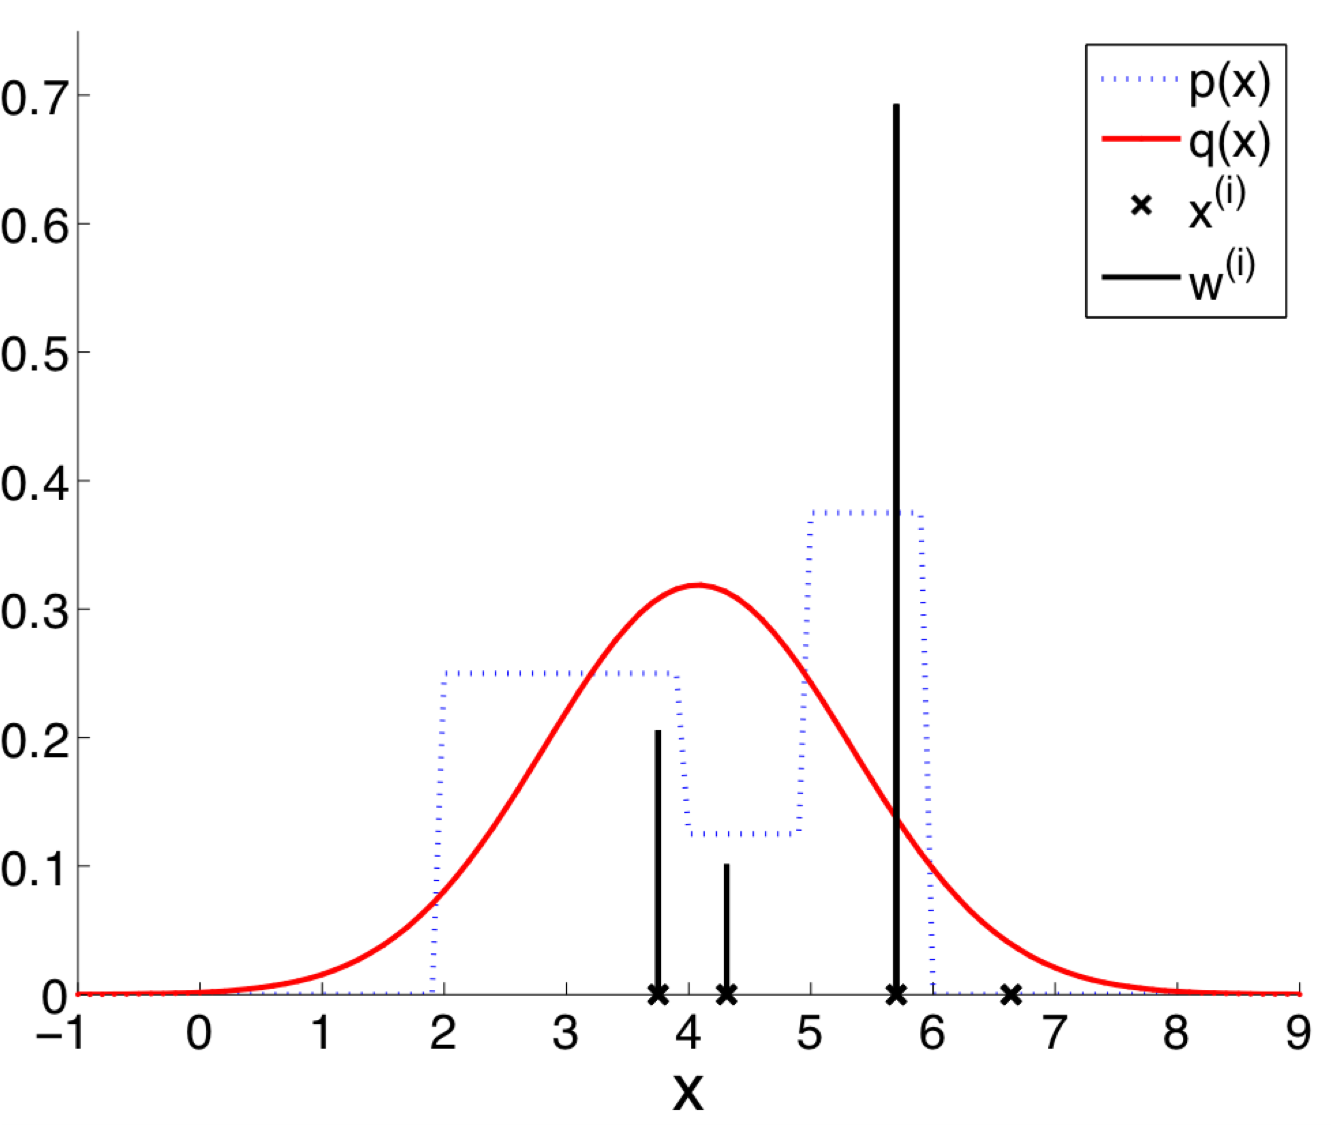
\includegraphics[scale=0.280]{img/particle_filters/P0_7_3_4_ex1.png}
\end{center}
\caption{Question figure.}
\label{P0_7_3_4_ex1}
\end{figure}
Perform resampling on the density and illustrate the result. Assume that the numbers 0.65, 0.03, 0.84 and 0.93 are drawn uniformly from $[0,1]$.
Which one of the following figures illustrates the resampled particles?

\begin{enumerate}
\item \begin{figure}[!htb]
\begin{center}
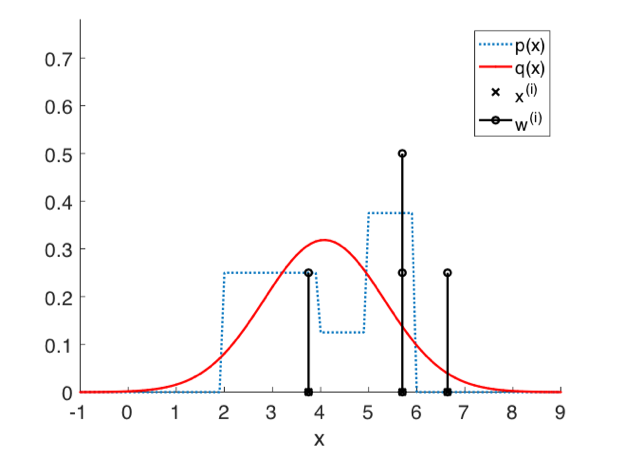
\includegraphics[scale=0.320]{img/particle_filters/P1_7_3_4_ex1.png}
\end{center}
\label{P1_7_3_4_ex1}
\end{figure}
\item \begin{figure}[!htb]
\begin{center}
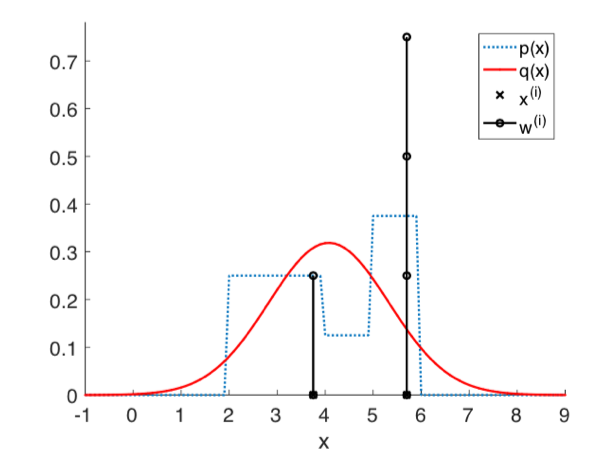
\includegraphics[scale=0.320]{img/particle_filters/P2_7_3_4_ex1.png}
\end{center}
\label{P2_7_3_4_ex1}
\end{figure}
\item \begin{figure}[!htb]
\begin{center}
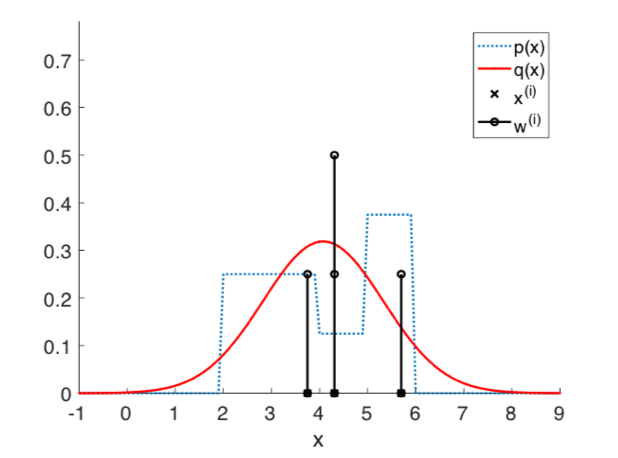
\includegraphics[scale=0.320]{img/particle_filters/P3_7_3_4_ex1.png}
\end{center}
\label{P3_7_3_4_ex1}
\end{figure}
\end{enumerate}
\item Bearing only tracking with a constant velocity motion in 2D, what is $\mathbf{x}_{k}^{l}, \mathbf{u}_{k}^{l}$ and $\mathbf{y}_{k}$ in this case

\begin{enumerate}
\item $\mathbf{x}_{k}^{l}$: position, $\mathbf{u}_{k}^{l}$: velocity, $\mathbf{y}_{k}$: bearing to target
\item $\mathbf{x}_{k}^{l}$: velocity, $\mathbf{u}_{k}^{l}$: position, $\mathbf{y}_{k}$: bearing to target
\item $\mathbf{x}_{k}^{l}$: velocity, $\mathbf{u}_{k}^{l}$: bearing to target, $\mathbf{y}_{k}$: position
\end{enumerate} 

\item Which of the following is true about the SIS (Sequential Importance Sampling) particle filter?

\begin{enumerate}
\item It outputs strictly Gaussian posterior distribution approximations. 
\item It can approximate multi-modal state distributions. 
\item It eventually degenerates to just a few particles with significant weights. 
\item It is a special case of a sigma-point filter. 
\end{enumerate}

\item With the particle filters we approximate the posterior as 
\begin{equation}
p(\mathbf{x}_k | \mathbf{y}_{1:k} \approx \sum_{i=1}^{N} w_{k}^{(i)}\delta(\mathbf{x}_k - \mathbf{x}_{k}^{(i)})
\end{equation}
Which of the following statements regarding this approximation are true?

\begin{enumerate}
\item $\mathbf{x}_k$ can take any value in $[\text{min}_i \mathbf{x}_{k}^{(i)},\text{max}_i \mathbf{x}_{k}^{(i)}]$
\item We can view this as a discrete distribution where $P(\mathbf{x}_{k} = \mathbf{x}_{k}^{(i)} | \mathbf{y}_{1:k}) = w_{k}^{(i)}$.
\item It follows that  $E[\mathbf{x}_{k} | \mathbf{y}_{1:k}] \approx \sum_{i=1}^{N} w_{k}^{(i)}\mathbf{x}_{k}^{(i)}$.
\item We can get arbitratry fine approximation by just in-creasing the number of particles, $N$ . 
\end{enumerate}

\item Consider Figure \ref{P6_importancesampling}

\begin{figure}[!htb]
\begin{center}
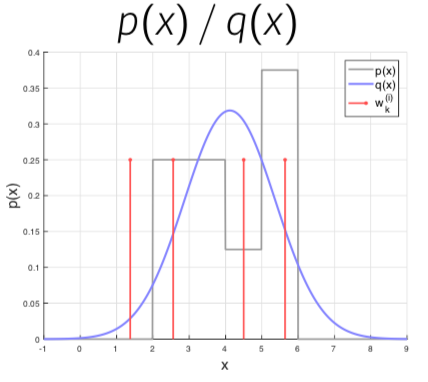
\includegraphics[scale=0.320]{img/particle_filters/P6_importancesampling.png}
\end{center}
\caption{Figure for exe}
\label{P6_importancesampling}
\end{figure}

Which one of the Figures \ref{P6a_importancesampling}, \ref{P6b_importancesampling}, \ref{P6c_importancesampling} and \ref{P6d_importancesampling} is the importance sampling approximation of $p(x)$ using $q(x)$ ?

\begin{enumerate}
\item \begin{figure}[!htb]
\begin{center}
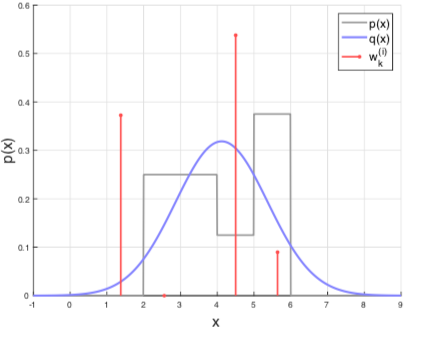
\includegraphics[scale=0.320]{img/particle_filters/P6a_importancesampling.png}
\end{center}
\caption{Option A}
\label{P6a_importancesampling}
\end{figure}
\item \begin{figure}[!htb]
\begin{center}
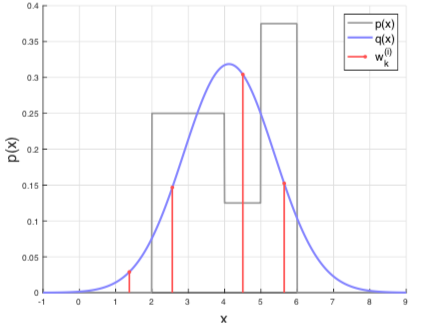
\includegraphics[scale=0.320]{img/particle_filters/P6b_importancesampling.png}
\end{center}
\caption{Option B}
\label{P6b_importancesampling}
\end{figure}
\item \begin{figure}[!htb]
\begin{center}
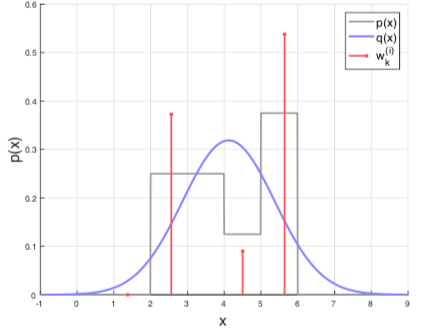
\includegraphics[scale=0.320]{img/particle_filters/P6c_importancesampling.png}
\end{center}
\caption{Option C}
\label{P6c_importancesampling}
\end{figure}
\item \begin{figure}[!htb]
\begin{center}
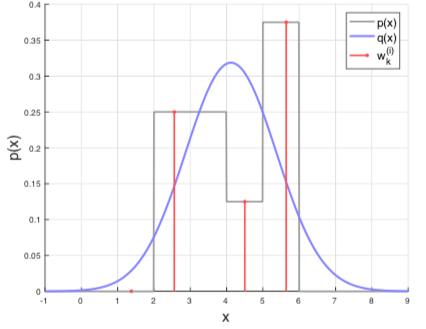
\includegraphics[scale=0.320]{img/particle_filters/P6d_importancesampling.png}
\end{center}
\caption{Option D}
\label{P6d_importancesampling}
\end{figure}
\end{enumerate}

\item Consider Figure \ref{P7_importancesampling}
\begin{figure}[!htb]
\begin{center}
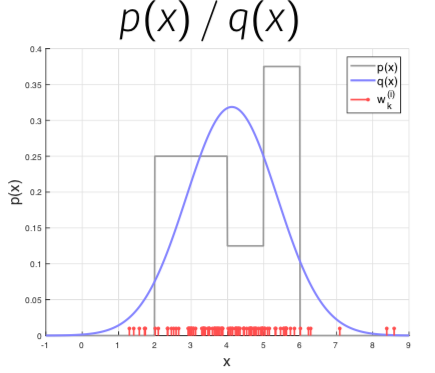
\includegraphics[scale=0.320]{img/particle_filters/P7_importancesampling.png}
\end{center}
\caption{Figure for exe}
\label{P7_importancesampling}
\end{figure}

Which one of the Figures \ref{P7a_importancesampling}, \ref{P7b_importancesampling}, \ref{P7c_importancesampling} and \ref{P7d_importancesampling} is the importance sampling approximation of $p(x)$ using $q(x)$ ?

\begin{enumerate}
\item \begin{figure}[!htb]
\begin{center}
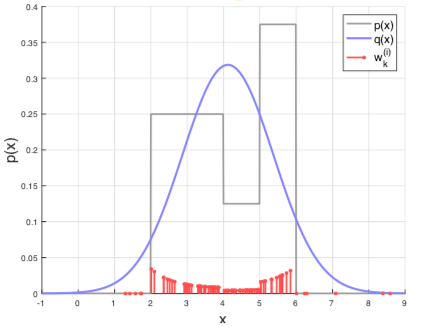
\includegraphics[scale=0.320]{img/particle_filters/P7a_importancesampling.png}
\end{center}
\caption{Option A}
\label{P7a_importancesampling}
\end{figure}
\item \begin{figure}[!htb]
\begin{center}
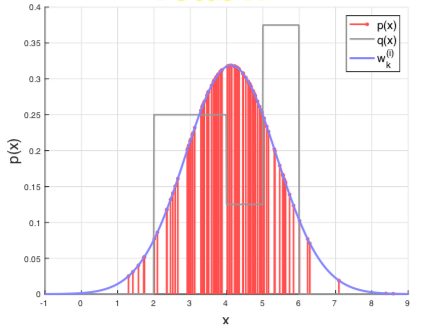
\includegraphics[scale=0.320]{img/particle_filters/P7b_importancesampling.png}
\end{center}
\caption{Option B}
\label{P7b_importancesampling}
\end{figure}
\item \begin{figure}[!htb]
\begin{center}
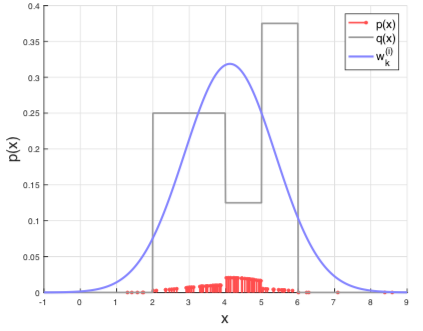
\includegraphics[scale=0.320]{img/particle_filters/P7c_importancesampling.png}
\end{center}
\caption{Option C}
\label{P7c_importancesampling}
\end{figure}
\item \begin{figure}[!htb]
\begin{center}
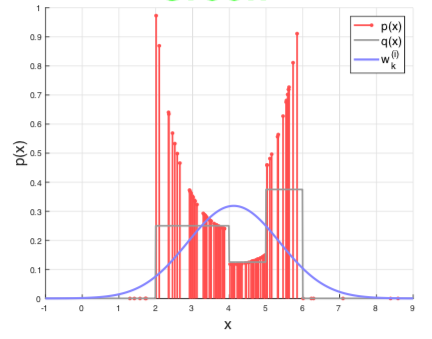
\includegraphics[scale=0.320]{img/particle_filters/P7d_importancesampling.png}
\end{center}
\caption{Option D}
\label{P7d_importancesampling}
\end{figure}
\end{enumerate}

\item Which of the following is true about the SIS (Sequential Importance Sampling) particle filter?

\begin{enumerate}
\item It outputs strictly Gaussian posterior distribution approximations. 
\item It can approximate multi-modal state distributions. 
\item It eventually degenerates to just a few particles with significant weights. 
\item It is a special case of a sigma-point filter. 
\end{enumerate}

\item Assume you want to compute the mean of a function $g(\mathbf{x})$ where $\mathbf{x}$ is distributed according to $p(\mathbf{x})$ which cannot
be sampled from. To compute an approximate mean, you use importance sampling with a proposal density $q(\mathbf{x})$ and the normalized
weights $w^{(i)}$.  What of the following is true?

\begin{enumerate}
\item The proposal density $q(\mathbf{x})$ must be proportional to $p(\mathbf{x})$
\item Samples $\mathbf{x}^{(i)}$ are drawn from $g(\mathbf{x})$
\item $p(\mathbf{x})$ is approximated by the samples $\mathbf{x}^{(i)}$ as $p(\mathbf{x}) \approx \frac{1}{N}\sum_{i=1}^{N}\delta(\mathbf{x}-\mathbf{x}^{(i)})$
\item The mean of any function $g(\mathbf{x})$ is approximated as $E[g(\mathbf{x})] \approx \sum_{i=1}^{N} g(\mathbf{x}^{(i)})w^{(i)}$
\item You must evaluate the densities $p(\mathbf{x}^{(i)})$ and $q(\mathbf{x}^{(i)})$ for each sample in order to compute the mean of $g(\mathbf{x})$ by importance sampling.
\end{enumerate}

\item Now you also want to compute the covariance of $g(\mathbf{x})$ . What of the following is true?

\begin{enumerate}
\item The proposal density $q(\mathbf{x})$ must have similar support as $g(\mathbf{x})$
\item Covariance of any function $g(\mathbf{x})$ can be approximated using importance sampling as $\text{Cov}(g(\mathbf{x})) = \sum_{i=1}^{N}\text{Cov}(g(\mathbf{x}^{(i)}))w^{(i)}$
\item When approximating the covariance of $g(\mathbf{x})$  using importance sampling, one can reuse the samples $\mathbf{x}^{(i)}$ and weights $w^{(i)}$ 
from when approximating $E[g(\mathbf{x})]$ with importance sampling.
\end{enumerate}

\item  What of the following is true about the SIR (Sequential Importance Resampling) particle filter?

\begin{enumerate}
\item It solves the degeneracy problem.
\item It should be performed at every time step. 
\item The number of samples reduces after resampling. 
\item Its performance depends on the quality of the importance distribtution. correct 
\item The bootstrap filter is a typical variation of SIR. 
\end{enumerate}

\item Which of the following statements regarding resampling are true?

\begin{enumerate}
\item By resampling we make an approximation of our particle approximation of $p(\mathbf{x}_k | \mathbf{y}_{1:k})$
\item By resampling we get a more accurate approximation of $p(\mathbf{x}_k | \mathbf{y}_{1:k})$ than what we had before we resampled.  
\item By resampling we move the particles in a similar manner as we do in the measurement update of a Gaussian filter. 
\item By resampling we focus our particles to high probability areas so they are not wasted in improbable states.  
\end{enumerate}

\item Resampling can sometimes result in lack of diversity.
Consider the following toy example: There are two rooms, and the robot is unsure about which room it is in. The non-informative sensor shows equal probability of being in either room. We start with N particles equally distributed between the two rooms. How are particles distributed after a sufficiently long time if resampling is done at each time step?

\begin{enumerate}
\item We don't know. It depends on the distribution of last time step. 
\item Each room will have the same number of particles. 
\item The particles will converge to one of the two rooms.   
\end{enumerate}

\end{enumerate}

\subsection{Assignements}


